\documentclass[12pt,a4paper]{report}
\usepackage[T1]{fontenc}
\usepackage[utf8]{inputenc}
\usepackage{charter}
\usepackage{ngerman}
\usepackage[left=2cm,right=2cm,top=2cm,bottom=2cm]{geometry}
\usepackage{amsmath}
\usepackage{amssymb}
\usepackage{tikz}
\usepackage{tabularx}

\begin{document}
	\section{Darstellungen von Automaten (23.08.24)}
	\subsection{Formal am Beispiel eines Kaugummiautomaten}
	\begin{align*}
		A &= \Bigl(Q, s, \Sigma, \Omega, \delta, \lambda\Bigl) \\
		Q & \ \ \ \text{Zustandsmenge}\ \ Q = \Bigl\{u, g\Bigl\}\ \ (\text{ungeladen, geladen})\\
		s & \ \ \ \text{Startzustand}\ \ s = u\\
		\Sigma &\ \ \ \text{Eingabealphabet}\ \ \Sigma = \Bigl\{M, H\Bigl\}\ \ (\text{Münze, Hebel})\\
		\Omega & \ \ \ \text{Ausgabealphabet}\ \ \Omega = \Bigl\{K, N\Bigl\}\ \ (\text{Kaugummi, Nichts})\\
		\delta &\ \ \ \text{Übergangsfunktion} \\
		&\ \ \ \delta: Q \times \Sigma \to Q\\
		&\ \ \ \ \ \ \ \ \delta(u,M) = g\\
		&\ \ \ \ \ \ \ \ \delta(u,H) = u\\
		&\ \ \ \ \ \ \ \ \delta(g,M) = g\\
		&\ \ \ \ \ \ \ \ \delta(g,H) = u\\
		\lambda &\ \ \ \text{Ausgabefunktion} \\
		&\ \ \ \lambda: Q \times \Sigma \to \Omega\\
		&\ \ \ \ \ \ \ \ \delta(u,M) = N\\
		&\ \ \ \ \ \ \ \ \delta(u,H) = N\\
		&\ \ \ \ \ \ \ \ \delta(g,M) = N\\
		&\ \ \ \ \ \ \ \ \delta(g,H) = K\\
	\end{align*}
	\subsection{Graph}
	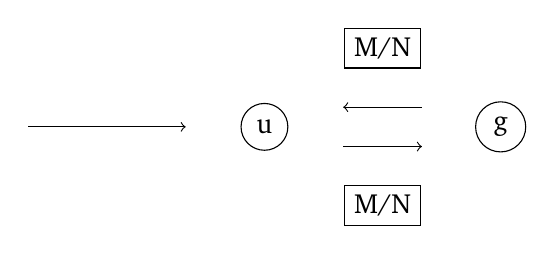
\begin{tikzpicture}
		\draw[->] (0,0) -- (2,0);
		\node at (3,0) [circle,draw]{u};
		\draw[->] (4,-0.25) -- (5,-0.25);
		\node[draw] at (4.5,-1) {M/N};
		\node at (6,0) [circle,draw]{g};
		\draw[->] (5,0.25) -- (4,0.25);
		\node[draw] at (4.5,1) {M/N};
	\end{tikzpicture}
	\subsection{Übergangstabelle}
	\begin{tabularx}{\textwidth}{|X|X|X|}
		\hline
		$\frac{\delta}{\lambda}$ & M & H\\
		\hline
		$u$ & $\frac{}{}$ & \\
		
		\hline 
	\end{tabularx}
\end{document}